\chapter{Shadowing in Sung Music and Human-Computer Interaction}
\label{chap:shadowing_in_sung_music_and_human_computer_interaction}

\lettrine{A} series of experiments is described in this chapter.
Some of them were designed to determine human behavior in \acl{hhi} and \ac{hci} as a mean of modeling interactions, and others examined the change in reactions of subjects to different adaptation strategies of implemented system as a subjective evaluation method.

\pagebreak

\section{Shadowing paradigm}
\label{sec:shadowing_paradigm}

In a shadowing task, participants are instructed to provide vocal productions as a reaction to pre-determined stimuli.
It is often used in empirical experiments \citep[e.g.,][]{Goldinger1998echoes} to examine how certain properties of these stimuli influence -- or do not influence -- participants' productions.
A shadowing task is typically preceded by a baseline phase, where the participants provide the same productions without listening to the stimuli.
The stimuli used in the shadowing phase can be determined based on the baseline production, e.g., for intentionally introducing a contrast between with respect to the participants' productions, as done in \cref{subsubsec:procedure_hci}.
A comparison between the production in these two phases indicates whether and to what extent the stimuli affected the participants' productions.
Sometimes a third, post-shadowing phase is added to examine whether the effect -- or lack thereof -- found in the shadowing phase remains when the external inputs are absent.
\Cref{fig:HCIConvFlow} shows a complete flow of the shadowing paradigm used in an experiment.
It is important to note that the baseline for change is not \SI{50}{\percent} (randomly retaining preferred realization or adopting stimulus' form).
Since people are not likely to spontaneously change their speech, the assumption here is that the probability of change represents the influence of the stimulus on the speaker.
More generally, the degree of accommodation can be seen as a speaker's tendency to converge to an interlocutor (cf.\ \emph{sensitivity} property in \cref{sec:parameters}).

Vocal accommodation is often studied using shadowing tasks, in which participants are asked to produce themselves utterances spoken by an interlocutor \citep[e.g.,][]{Pardo2018comparison, Babel2014novelty, Shockley2004imitation, Walker2015repeat, Dias2016visibilivty, Dias2016visibilivty}.
\todo[inline]{need anything else from shadow article (lines 402 on)?}
The ability to present specific contrasts and measure production differences in a controlled fashion makes it suitable for such studies.
However, this method also has some disadvantages.
One drawback is that while it is suitable for a controlled experimental environment, it only loosely represents a real-world conversation, due to the lack of utterance unpredictability, turn-taking, defined common goal, and more.
Another potential hindrance is that participants might tend, intentionally or not, to imitate the stimuli, which may lead to a false effect of high convergence that does not represent the participants' natural behavior.
This should be addressed in the experimental design and the instructions are given to the participants, e.g., by not making the target features too obvious and by not using wordings like \enquote{repeat}, \enquote{mimic}, or \enquote{like you heard} in the instructions.

A distinction can be made between two types of shadowing:
In \emph{Close shadowing}, participants start their production while a stimulus is still being played.
This means that they need to deal with both generation and processing at the same time.
\emph{Consecutive shadowing}, on the contrary, requires participants to listen to a stimulus in its entirety after it is finished.
This becomes harder the longer a stimulus is, merely due to the increasing difficulty to remember long segments.
Both of the experiments presented in this chapter use consecutive shadowing.
The simulated \ac{hci} experiment (\cref{sec:convergence_to_natural_and_synthetic_stimuli}) uses short sentences with which the participants are already familiar from the baseline phase. 
In the sung music experiment (\cref{sec:alignment_in_novel_and_familiar_sung_music}) the musical pieces are relatively long, and the analyses accounted also for parts that the participants did not produce (due to memorizing difficulties or otherwise).

\section{Prosodic alignment in novel and familiar sung music}
\label{sec:alignment_in_novel_and_familiar_sung_music}

\todo[inline]{motivation to do this experiment. relation and differences to linguistic accommodation}
As further explained in \citet{Raveh2020SpeechProsody}, 

\todo[inline]{specifically, see if there is something that can be taken from the abstract}

% how relates to vocal accommodationa in general and HHI experiment. -- gives the aspect of accommodation occuring not only in speech, but other vocal communications as well.
% things common to music and speech

Since both speaking and singing are used in social contexts, external factors may potentially affect them.
This enables, among other things, convergence effects between people productions.
In the case of music, convergence can be expressed in different aspects than in speech, like singing more accurately, shifting the musical key, adapting to a different tempo, etc.
%Furthermore, seeing that the tonal targets in singing are pre-defined, there are precise targets for production -- either from a heard example or from one's mental memory -- in an experimental setting.
%Therefore, the participants' productions can be directly compared with some \enquote{ground truth}.

The rhetorical aspects of music and spoken language can be described in musical terms.
These two vocal capabilities share some properties in both production and perception.
Such common properties include articulation rate, intensity, timbre, and others.
Moreover, intonation, pitch, timbre, rhythm, and tempo are all common in descriptions of music, as they are in speech \citep{Molino2000toward, Jackendoff2009parallels}.
Similarly, \citet{Day2013speech} also shows how some phenomena related to spoken language can also be described using musical means.
Another important aspect is that both have a temporal dimension and evolve over time.
However, music usually consists of defined \emph{absolute} pitch and rhythmic targets.
This is even more salient when dealing with familiar musical materials, as both the singer and the listener are already primed as to what they expect to hear before listening \citep{Meyer2008emotion}.
In speech, on the other hand, the phonetic features of a specific utterance are not expected to match specific absolute values.
These similarities and differences between spoken language and music raise the question of whether vocal convergence occurs in music production as well.
Since the focus here is on vocal changes, sung music was examined in the study.
However, to prevent influences due to the phonetic properties of specific words, the singing was performed without lyrics (see \cref{subsubsec:procedure_music}).

The main research question of the study presented here is whether convergence occurs in singing as well, and, if so, whether specific parts of the musical piece are prone to changes.
%Our hypothesis is that convergence will be found in the participants' performances with respect to the pre-recorded stimuli.
Convergence can be realized on the absolute level, meaning that the participants shift their overall pitch range (the \emph{key}) and tempo to be closer to the recording, or relative to their own singing by making the pitch and temporal intervals between the target notes more precise after listening to the recording.
A secondary research question is how the familiarity with the musical material affects reproduction.
The expectation here is that the participants' performances of the familiar lullaby will be accurate even before listening to a version of it in terms of deviation from the target intervals, but even more so afterwards.
When reproducing an unfamiliar melody, it is not expected that the participants will remember it in its entirety, but rather that they would stick to repeating segments or parts with smaller intervals and simpler rhythms.
Additional background and motivations can be found in \citet{Raveh2020SpeechProsody}.

%The experimental procedures and materials are described in \cref{sec:method}.
%\cref{sec:analysis_music} presents the methods applied to analyze the prosodic properties \emph{pitch}, \emph{tempo}, and \emph{rhythm}.
%%These are the two main features that are directly noted in musical sheets, and play an important role in both speech and music and have been studied in speech convergence studies \citep{Schweitzer2013convergence}.
%Results are presented in \cref{sec:results}, along with some representative examples from the participants' performances.
%Finally, interpretations and additional observations are discussed in \cref{sec:discussion_and_conclusion}, which also concludes the paper.

\subsection{Experimental design}
\label{subsec:design_music}

\subsubsection{Target features}
\label{subsubsec:target_features_music}

Phonetic convergence in speech has been studied with respect to various prosodic features, such as speech rate \citep{Schweitzer2013convergence, Pardo2012phonetic}, \ac{f0} \citep{Babel2012role, Collins1998convergence}, intonation \citep{DImperio2014phonetic, Simonet2011intonational}, rhythm \citep{Krivokapic2013rhythm}, and more.
The study presented here deals with the musical prosodic features \emph{tonal deviation} (perceived \ac{f0} difference), \emph{rhythmic precision} (with respect to specific rhythmic patterns), and overall tempo and key choice.
The latter two are global properties and were determined based on an entire performance.
In \cref{subsec:results_music} it is explained how these features were measured in music, where the tonal and rhythmic targets are defined based on a musical theoretical framework.

\subsubsection{Procedure}
\label{subsubsec:procedure_music}

The study consists of two shadowing experiments (see \cref{sec:shadowing_paradigm}).
The first experiment examined convergence effects between the two performances of the participants.
The participants were first asked to sing the familiar Yakinton's melody with the syllable \textipa{[na]} instead of its lyrics (regardless of whether the participant could, de facto, recall the lyrics).
Besides that, no specific instructions were given, e.g., regarding the tempo, the key, or any other musical preference.
Subsequently, the participants listened to the pre-recorded version of the lullaby via wired over-ear headphones. %(Phillips SHL3060).
Following that, they sang the lullaby once more and answered some questions regarding the recorded version of the lullaby, to determine how much it differs from the one in their mental memory.
Importantly, no reference to either their previous production or the recorded version was made by using wordings like \enquote{repeat}, \enquote{mimic}, \enquote{like before}, etc.
The second experiment comprised only a shadowing performance, as the participants were intentionally unfamiliar with the universal lullaby.
This experiment tests which prosodic features would be replicated more accurately when it is not likely that the participants would remember all aspects of the musical material.
After listening to the pre-recorded version of the lullaby, they were instructed to sing it themselves to the best of their ability.
This required not only their singing capabilities, but also their musical memory.
As explained above, this lullaby was composed using universal characteristics of the genre and should therefore contain similar melodic and harmonic contents to the lullaby in the first experiment.
The two experiments were carried out consecutively.
In addition to the short questions in the first experiment, the participants also answered a personal questionnaire before starting the second experiment and a closing questionnaire at the end.
The entire procedure lasted \SIrange{15}{20}{\minute} in total per participant (and see \citet{Raveh2020SpeechProsody} for further details).

\subsubsection{Material and participants}
\label{subsubsec:material_participants_music}

\begin{snippet}[t]
	\centering
	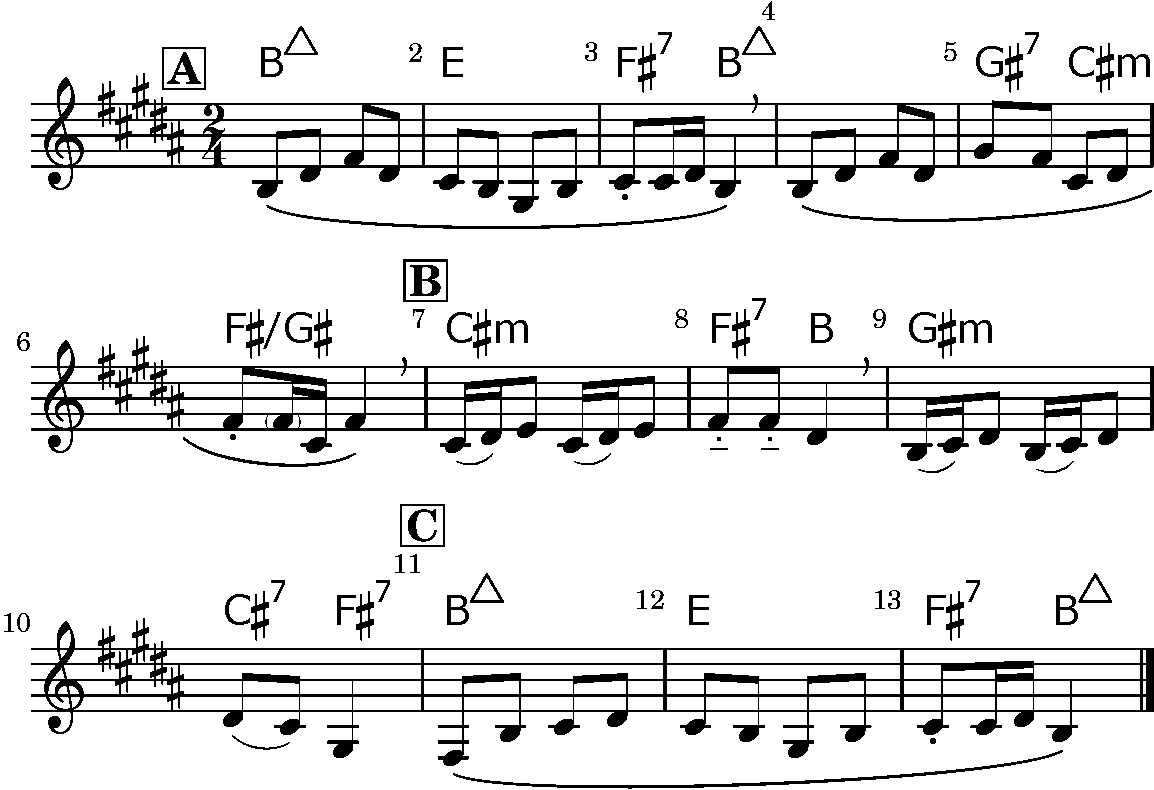
\includegraphics[width=0.8\linewidth]{yakinton}
	\caption[Yakinton lullaby]
		{The Yakinton lullaby transposed to B major.
		The square labels \enquote{A}, \enquote{B}, and \enquote{C} mark the \emph{theme}, \emph{bridge} (or \emph{development}), and \emph{recapitulation} sections of the lullaby.
		The breath marks are placed where the participants are expected to make a brief break and/or lengthen the ending of a phrase.
		The first sixteenth note in bar six is in brackets since it is not present in the original melody and was therefore also excluded in the recorded version played to the participants.
		However, it is common to add it, and indeed all participants included it in both performances.}
	\label{snippet:yakinton}
	\addcontentsline{lof}{section}{Snippet \thesnippet: Yakinton lullaby}
\end{snippet}
%
Sung lullabies were chosen in this work, as they are more memorable than other musical genres and than instrumental pieces \citep{Weiss2012something, Trehub1991music}, especially among mother to small babies, as those that took part in the study (see below).
Two lullabies were used in the study, one for each experiment: The first is \enquote{Tune for the Yakinton}\footnote{Pizmon LaYakinton
% (\emph{Hebrew:}\hebrewtext{פזמון ליקינטון})
, written by Leah Goldberg in 1940. \emph{Yakinton} is the Hebrew name of the Hyacinth plant.} (hereafter \enquote{Yakinton}, see \cref{snippet:yakinton}), which is a famous Israeli children lullaby.
The second is a culturally universal lullaby composed for experimental purposes \citep[][pp.~22-47, and see \cref{snippet:uni-lullaby}]{Twig2016universal}, which contains \emph{cross-cultural characteristics}, like repetitiveness, simple melody, and a limited inventory of tonal and rhythmic patterns \citep{Unyk1992lullabies, Trehub1993maternal}.
Therefore, while the first one is assumed to be known to the participants, they could not be familiar with the second one.
Both lullabies are short (13 bars at \musQuarter~=~61 ($\approx$\SI{26.5}{\second}) and 16 bars at \musQuarterDotted~=~33 ($\approx$\SI{58}{\second}), respectively) and in major keys.
The lullabies were recorded a cappella by a trained female singer in the same age group as the participants in a professional recording studio at \SI{44.1}{\kilo\hertz} sampling rate and 16-bit resolution.
To avoid changes in voice production, decrease vibrato, and limit the singing effort, they were both transposed and recorded in B major, which is relatively low for female voices.
\todo{need a footnote here to explain why the transposition helped with these things?}
This also prevents influences originating from the use of a different key in each lullaby recording.
The syllable \textipa{[na]} was used throughout the lullabies in both recorded versions instead of any lyrics to eliminate biases due to their lyrics or the realizations of specific sounds.
This way, the possibility that participants would hesitate in their performances because they know the melody but not the lyrics was avoided as well.
%
\begin{snippet}[t]
	\centering
	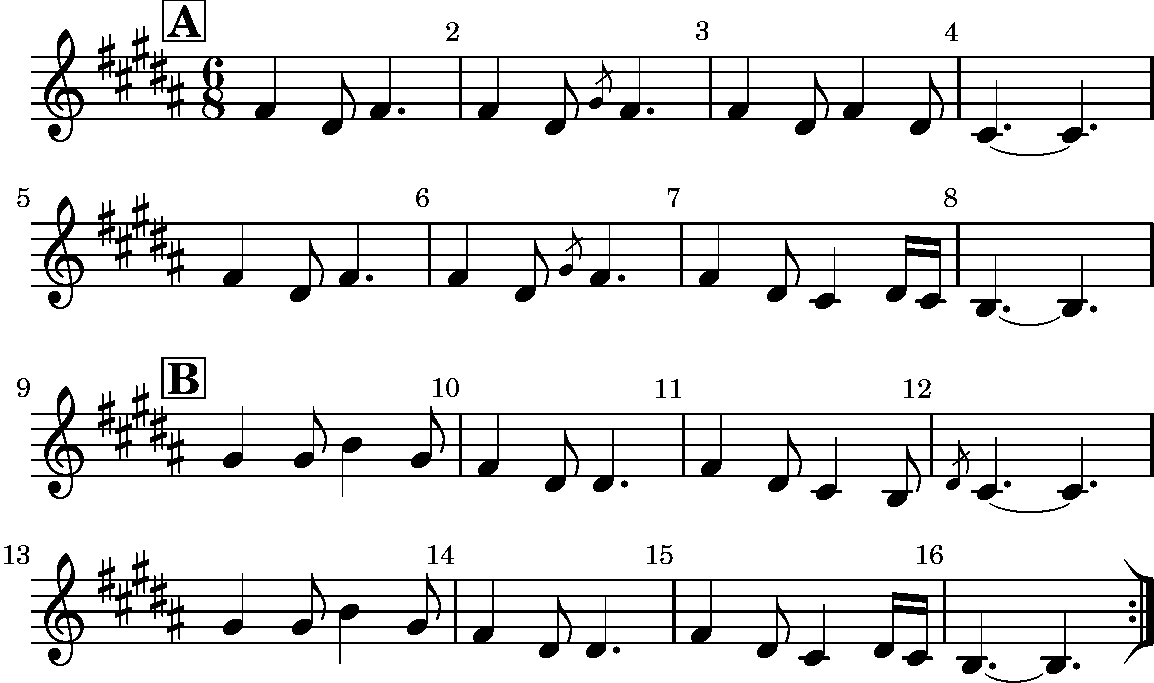
\includegraphics[width=0.8\linewidth]{lullaby}
	\caption[Universal lullaby]
		{The universal lullaby.
		The square labels \enquote{A} and \enquote{B} mark the structural parts.
		The grace notes in bars 2, 6, and 12 were included in the recording but due to their secondary melodic role did not penalize performances that lacked them.}
	\label{snippet:uni-lullaby}
	\addcontentsline{lof}{section}{Snippet \thesnippet: Universal lullaby}
\end{snippet}
%

Six participants took part in the study, all of which are mothers to recently born babies and with no hearing impairments.
For three of the mothers, this was the first child.
Their age ranged from 29 to 37 years (mean 35.5~$\pm$3.25) and the age of their babies ranged from one to seven months (mean 4.5~$\pm$3.5).
To further homogenize the participants' characteristics, and their musical education and experience were controlled as well.
None had any professional-level musical background and four disclosed they have been singing or playing an instrument recreationally.
Since singing is a skill that can be methodically improved, it was required to find participants with no professional-level singing skills on the one hand, but still sing regularly in a social context \emph{without the direct goal of improving their singing quality}.
To that end, mothers who reported that they sing to their new-born babies were selected.
In the pre-verbal phase, parents often sing to their babies.
When communicating with infants, adults tend to use exaggerated prosody with elevated melodic pitch and distinct rhythmic patterns \citep{Fernald1991prosody}.
The increased use of singing as well as its function as a means of communication with their babies \citep[see][]{Street2003mothers,Papouvsek1991meanings} made mothers of small babies suitable for this study.
Since the participants' singing capabilities are essential for their performances in the experiments, it was also confirmed that they regularly sing lullabies for their babies.
Furthermore, as we are dealing with a specific lullaby in the first experiment, their familiarity with it was confirmed.
All the participants reported that they know the Yakinton lullaby well enough to spontaneously sing it from memory.

\subsection{Analyses and results}
\label{subsec:results_music}

Since the participants aimed to produce specific musical notes (as opposed to non-specific absolute frequencies in speech production), tones were used for measuring pitch instead of raw Hertz values.
For that, quarter tones (\acfp{qt}) were used instead of semitones to increase the tonal resolution, 
Using \acp{qt} rather than traditional half-tones enables a more fine-grained analysis that can capture more subtle off-key singing and differentiate the performances better.
%The performances were manually transcribed in Sibelius 6
%\todo{version footnote}
%and were verified using the corresponding MIDI output against the recordings.
%
\begin{figure}[t!]
	\centering
	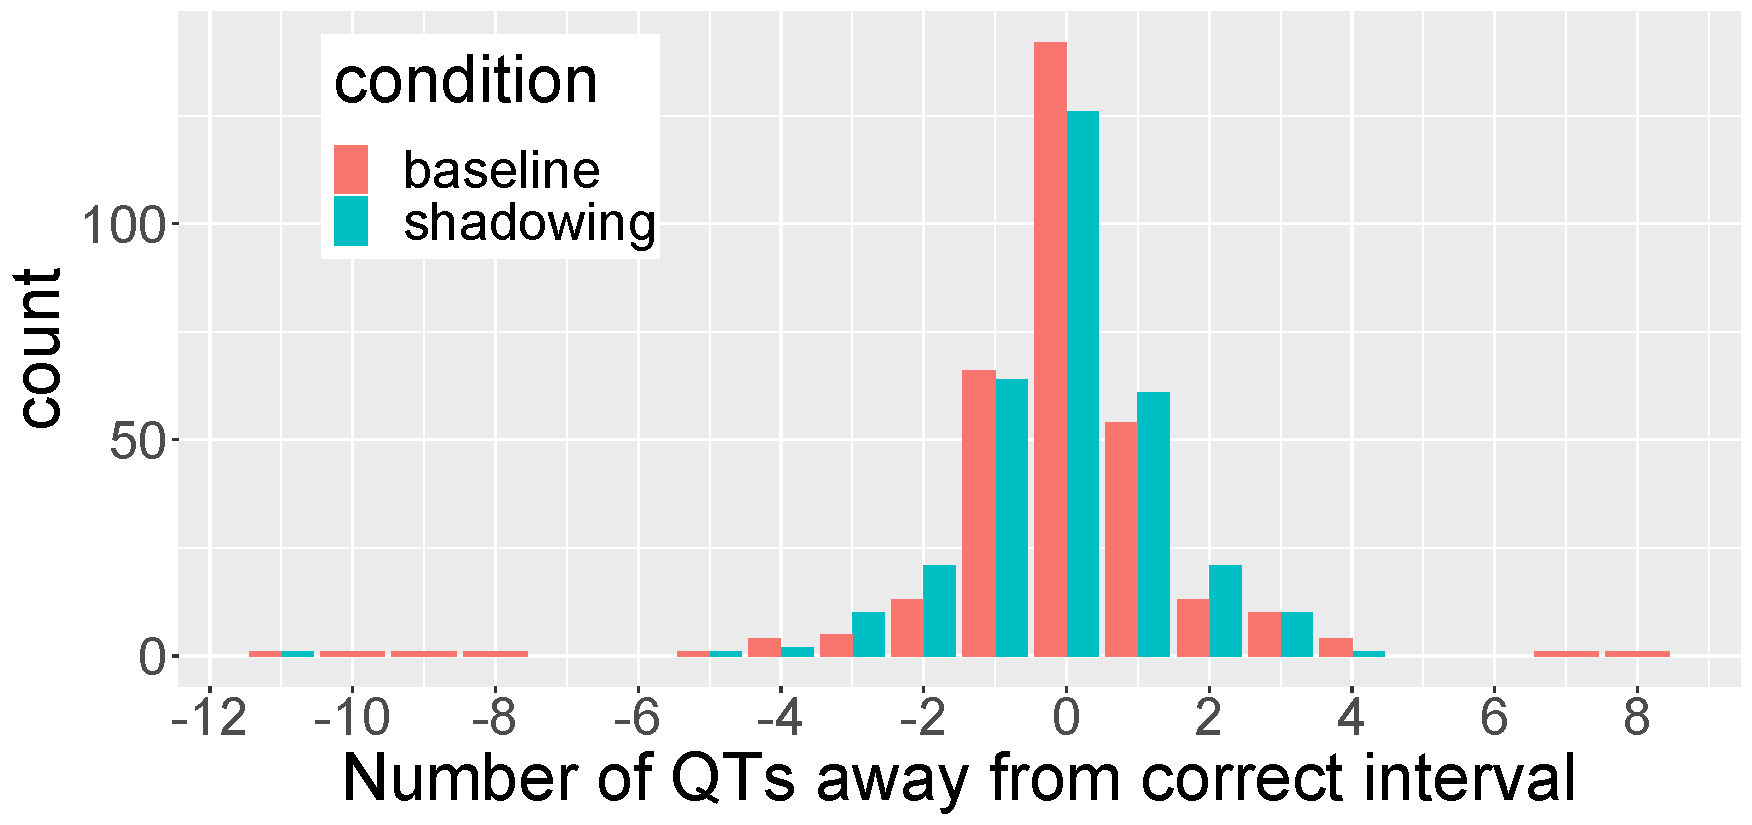
\includegraphics[width=\linewidth]{barplot_QT_distances}
	\caption[Violin distributional comparison of participants' singing deviations in both phases]
		{A comparison between each participant's distribution of deviations in both phases.
		 The width of the violin shape indicates the counts of the \acsp{qt} deviations.
		 The upper and lower hinges of the white boxes within the violin shapes show the first and third quartiles, with the thick black line marking the median value.
		 The vertical line crossing the white box show the value range, excluding outliers.}
	\label{fig:barplot_QT_distances}
\end{figure}
%
The segmentation of the performances into individual tones was done manually by a trained musician.
Silences, non-singing, breaths between phrases, etc.\ were segmented as well.
The tone frequencies were determined by the median of the measured frequencies during this tone's duration, excluding the first and last \SI{10}{\percent} of the tone duration.
This excludes transitions between tones and smooths out vibrato and ad lib ornaments.
These values were extracted using Praat \citep{Boersma2018praat} with manual corrections where necessary.
Subsequently, the note assigned to each singing segment was determined by selecting the closest \ac{qt} to the measured frequency in the corresponding segment.
This stands in line with the assumption that people sing with a specific tone in mind rather than a frequency.
The mapping between tone frequencies and \acp{qt} (relative to middle A) was done using the formula
%
\begin{equation}
	\label{eq:quarter_tones_formula}
	frequency(QT_n) = 440 \cdot \sqrt[24]{2}^n,
\end{equation}
\eqname{\Acl{qt} frequency calculation (equal temperament)}\noindent
%
where $n$ is the number of \acp{qt} away from the middle A tone \citep[cf.][]{DeKlerk1979equal} and \SI{440}{\hertz} is the frequency of the middle A based on the equal temperament.
%, which can be assumed to be the tuning system with which the participants grew up.
QTs are denoted here with the symbols \hspace{-0.26cm}
$\vcenter{\hbox{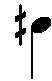
\includegraphics[height=15pt]{qt_c-cih}}}$ and 
$\vcenter{\hbox{
\includegraphics[height=15pt]{qt_c-cisih}}}$ for one \ac{qt} and three \acp{qt} above a note, respectively.
Ultimately, tonal deviations were measured per interval, rather than per tone, as the latter would depend on the key the participants chose, while the former measures tonal accuracy independently of a key.
Tempo was measured for an entire performance, taking into account only singing segments (similarly to measuring \ac{ar} in speech).
This ensures that pauses between phrases do not influence the perceived singing tempo and that occasional, non-written lengthenings (e.g., short ritardandi and fermate at the end of phrases) do not mark a specific note as being out of rhythm.
Tempo was measured in \acf{bpm}, which is directly derived from the standard musical notation \musQuarter~=, using the formula
%
\begin{equation}
	\label{eq:bpm}
	BPM = \frac{N + \delta}{overall\ duration} \cdot 60,
\end{equation}
\eqname{\Acf{bpm}}\noindent
%
where $N$ is the number of beats in the lullaby and $\delta$ is the number of beats, if any, added by a participant.
Such additions occurred exclusively at the end of phrases (bars 3, 6, 10, and 13 in \cref{snippet:yakinton}), but are not present in the pre-recorded stimulus.
The Yakinton lullaby (\cref{snippet:yakinton}) and the universal lullaby (\cref{snippet:uni-lullaby}) have 26 quarter beats and 32 dotted quarter beats, respectively.

As expected, the participants could, for the most part, accurately produce the Yakinton lullaby (\cref{snippet:yakinton}) based merely on their memory in the baseline phase.
However, as \cref{fig:barplot_QT_distances} shows, these performances included several large deviations of two tones or more, which are not likely to be caused by coincidental imprecise singing.
In the shadowing phase, in comparison, there was only one such large deviation.
This adjustment of obviously wrong tones was presumably driven by the exposure to a correctly sung version.
Other than these corrections, the deviation distributions shown in \cref{fig:barplot_QT_distances} are roughly symmetric and similar in both phases.
Surprisingly, the baseline performances had more correct tones as a whole.
It seems, therefore, that the reference version helped the participants to sing within a more accurate range of tones, but somewhat eroded their precision in some notes.
To confirm that the changes were subtle and were ascribed mostly to larger deviations, a distributional comparison between the baseline and shadowing productions for each participant.
These comparisons are shown in \cref{fig:violin_facet_dev}.
The very high statistical distribution similarity results tests confirm that all participants didn't substantially change their singing, but in most cases, the deviation distribution in the shadowing phase was less scattered.
%
\begin{figure}[t!]
	\centering
	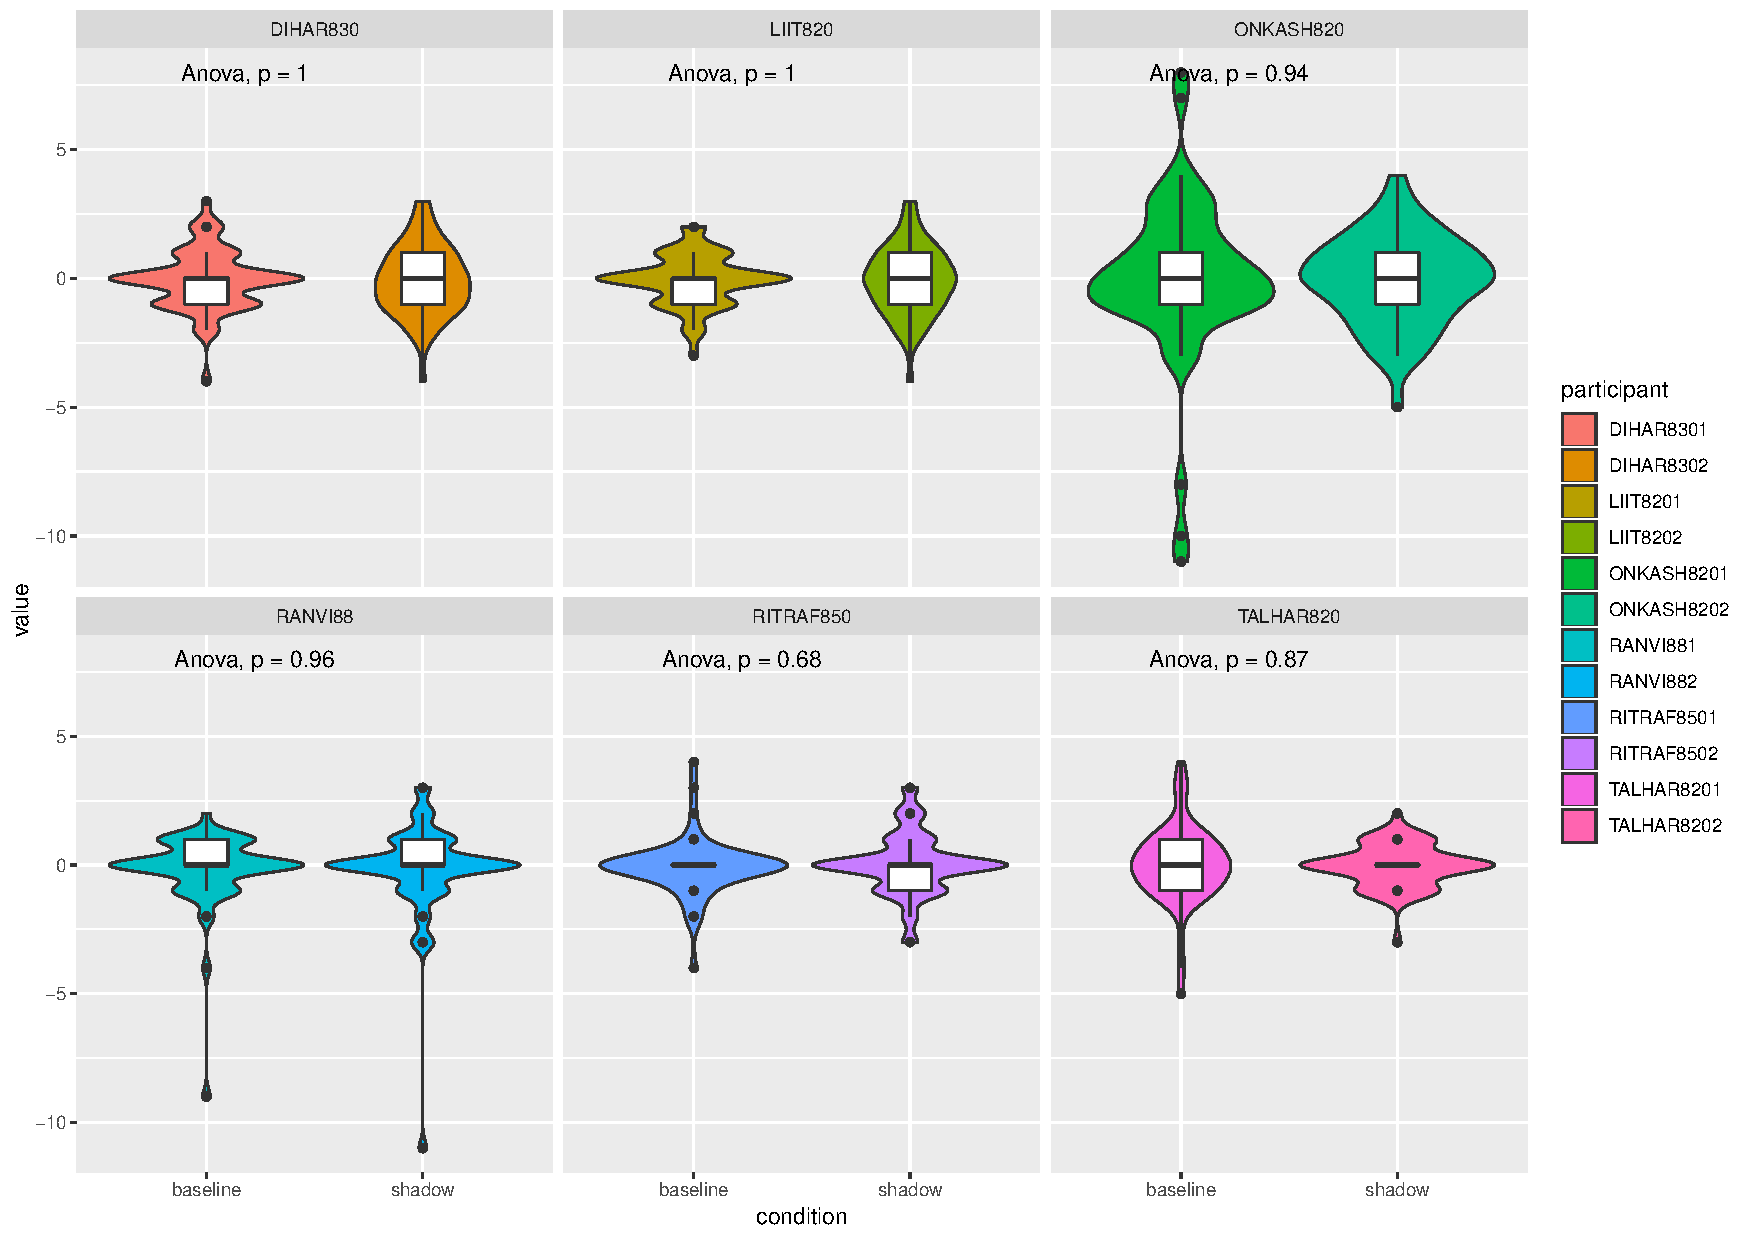
\includegraphics[width=\linewidth]{violin_facet_dev}
	\caption[Summary of within-participant interval deviation distribution]
		{Comparison between the distribution of deviations from the correct intervals in baseline (red) and shadowing (blue) performances.
		The numbers on the x-axis are the number of \acp{qt} above or below the correct interval.}
	\label{fig:violin_facet_dev}
\end{figure}
%
\begin{figure}[t]
	\centering
	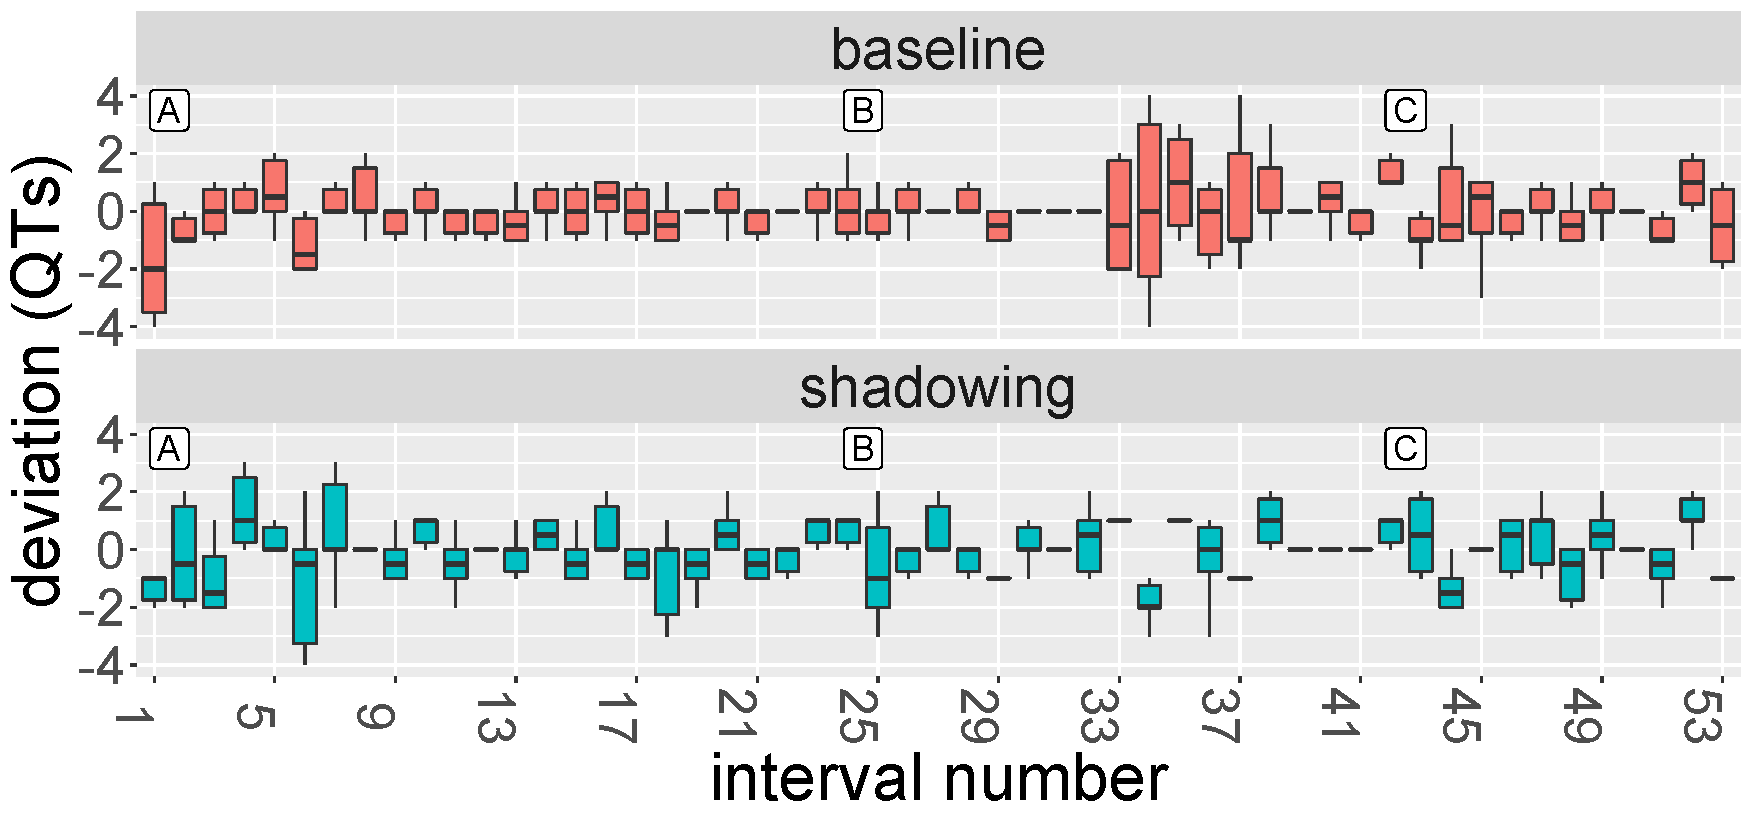
\includegraphics[width=\linewidth]{barplot_facet_tone_diff}
	\caption[Comparison of interval deviation between baseline and shadowing performances]
		{Comparison between the deviation distribution of each interval in baseline (top) and shadowing (bottom) conditions.
		The numbers on the x-axis are the interval indices representing the 53 intervals in the Yakinton lullaby.
		The distances between the intervals sang by the participants and the correct intervals are shown on the y-axis (outliers are omitted).
		The labels \enquote{A}~to~\enquote{C} mark the different parts of the lullaby (and correspond to the same labels in \cref{snippet:yakinton}).}
	\label{fig:barplot_facet_tone_diff}
\end{figure}
%
The tone-by-tone comparison presented in \cref{fig:barplot_facet_tone_diff} sheds more light on these differences.
It is evident that except for the very first interval, the participants showed greater consecutive variation in the second part of the bridge (label \enquote{B} in \cref{snippet:yakinton}, notes 34 to 42), while in the shadowing condition the first phrase (first seven intervals) showed a similar tendency.
Although the bridge moves to a new tonal center, it is not clear why only its second part would cause the singers to be less precise.
As for the higher variation at the beginning of the shadowing performances, this points to the process of re-finding the right tones in the participants' key of preference.
This explanation is supported by the key comparisons in \cref{tab:bpm_and_keys}, which show that there was virtually no key change between the baseline and shadowing performances by any of the participants.
Despite that, the unstable beginning of the shadowing performances indicates that listening to the recorded version influenced the participants' tonal accuracy.
This stands in line with the claim that also in speech, the beginning of a conversation is most prone to inter-speaker influences \citep[e.g.][]{Orlob2018nine}.
Participants needed about one whole phrase to overcome this influence and enter their preferred tonal center anew.
Interestingly, the only participant who sang in the same key as the recording did change key in the second performance.
The accuracy of tonal replication was measured in two ways, viz.\ directionality and quantity.
First, the correctness of the contour direction in each interval was evaluated (higher tone, lower tone, or same tone).
Second, the size of each interval was compared with the correct interval.
The participants correctly produced the contour direction in \SI{70}{\percent} of the intervals they replicated.
The intervals themselves, however, were correct only in \SI{44}{\percent} of the time.
This suggests that the overall contours of the lullaby are more easily recalled than the specific intervals.
\cref{snippet:deviation_examples} shows concrete examples of tonal and rhythmic deviations and \cref{snippet:deviation_example} shows the average deviations of all productions
%
\begin{table}
	\caption[Key and \acs{bpm} deviation summary]
			{Comparison between the singing tempo and key in baseline and shadowing performances of each participant.
			The values on the left and right under the key and \acs{bpm} columns are for baseline and shadowing performances, respectively.
			\acs{bpm}$\Delta$ shows the \acs{bpm} difference between baseline and shadowing, with the value in parentheses standing for the change in the difference from the recording's tempo.
			A negative value means that the participant decreased the distance to the recording.}
	\label{tab:bpm_and_keys}
	\centering
	\begin{tabularx}{\linewidth}{Xccc}
		\toprule
		\bfseries{Participant}	& \bfseries{Key}			& \bfseries{\acs{bpm}}		& \bfseries{\acs{bpm}$\Delta$}	\\
		\midrule
		RITRAF85				& F  |  F$\sharp$			& 76  |  70					&  6 ($-$6)						\\
		TALHAR82				& B  |  B$\flat$			& 57  |  63					&  6 ($-$2)						\\
		RANVI88					& A  |  A					& 59  |  63					&  4 (\phantom{$-$}0)			\\
		ONKASH82				& F$\sharp$  |  F$\sharp$	& 76  |  69					&  7 ($-$7)						\\
		LIIT82					& F$\sharp$  |  F$\sharp$	& 59  |  66					&  7 ($+$3)						\\
		DIHAR83					& F$\sharp$  |  F$\sharp$	& 62  |  61					&  1 ($-$1)						\\
		\rule{0pt}{0.5cm}% 
		recording				& (B) | B					& (61) | 61					&								\\
		\bottomrule
	\end{tabularx}
	\todo[inline]{any numeric values that can be put for key (e.g., difference in quartertones)}
\end{table}
%
\begin{table}[b]
	\caption[Percentages of rhythmic pattern replications]
		{Comparison between the percentage of occurrences of each rhythmic pattern in the original and replicated versions in all bar-level patterns.
		Parts A and B refer to the labels with the same letters in \cref{snippet:uni-lullaby}.
		Each replication row refers to the average over all participants who replicated that part.}
	\label{tab:neutral_rhythm_key}
	\centering
	\begin{tabularx}{\linewidth}{XSSSS}
		\toprule
						& \bfseries{R1}		& \bfseries{R2}		& \bfseries{R3}		& \bfseries{R4}\\
		\midrule
		original part A	& 50				& 12.5				& 12.5				& 25\\
		replications A	& 54				& 18				& 7					& 21\\
		\rule{0pt}{0.5cm}%
		original part B	& 25				& 37.5				& 12.5				& 25\\
		replications B	& 25				& 42				& 8					& 25\\		
		\bottomrule
	\end{tabularx}
\end{table}
%
The tempo of the recorded version is \SI{61}{\ac{bpm}}.
In their baseline performances, three participants sang faster than that and three more slowly.
All participants changed their tempo so that it was closer to the recorded version (see \cref{tab:bpm_and_keys}).
Moreover, the absolute distance from the recording's tempo decreased in all cases but one, which shows an alignment effect.
In contrast to the first lullaby, it was not expected that participants would be able to completely replicate all rhythmic patterns in the second lullaby (\cref{snippet:uni-lullaby}).
Two participants managed to replicate part A, part B was replicated by three participants, and one participant replicated both parts.
The replication rate of each rhythmic pattern was measured separately.
\Cref{tab:neutral_rhythm_key} summarizes the occurrences of the rhythmic patterns (R1--R4, corresponding to the rhythmic patterns in bars 5, 9, 15, and 16 in \cref{snippet:uni-lullaby}, respectively) in the original and replicated versions.
The proportion of each pattern within a part was generally preserved in the participants' performances, with the expected occasional confusions between R2 and R3 in part A due to their difference only in the last third beat that may be interpreted as a stylistic choice.
It is also evident that R1 and R4 were replicated more accurately.
An explanation for that is their simplicity compared to R2 and R3 and that they appear at the beginning and end of every phrase, making them easier to remember.
They contain fewer tones (and thus intervals) than R2 and R3.
%
\begin{snippet}[t]
%	\centering
	\begin{minipage}{.41\linewidth}
		\centering
		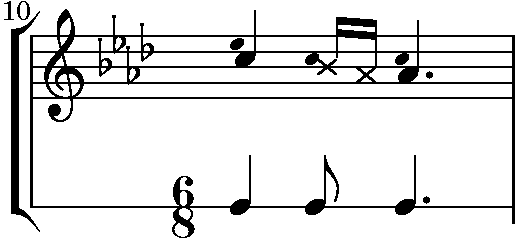
\includegraphics[width=\linewidth]{deviation_example_1}
	\end{minipage}%
	\hfill
	\begin{minipage}{.49\linewidth}
		\centering
		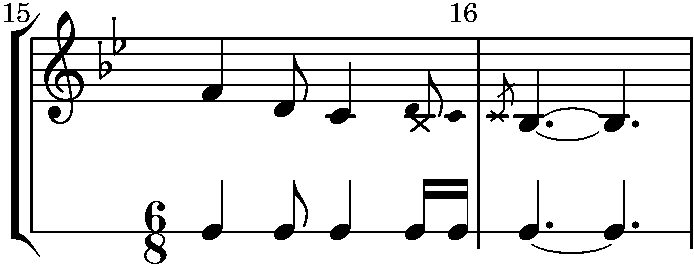
\includegraphics[width=\linewidth]{deviation_example_2}
	\end{minipage}%
	\caption[Examples of tonal and rhythmic deviations]
		{Examples of tonal (top staff) and rhythmic (bottom staff) deviations in bar 10 (left score) and bars 15-16 (right score) of the universal lullaby.
		Smaller, stemless notes mark the correct notes where deviation occurred.
		Crossed-head notes mark those that deviate from the correct rhythmic pattern.}
	\label{snippet:deviation_examples}
	\addcontentsline{lof}{section}{Snippet \thesnippet: Examples of tonal and rhythmic deviations}
\end{snippet}
%
\begin{snippet}[H]
	\centering
	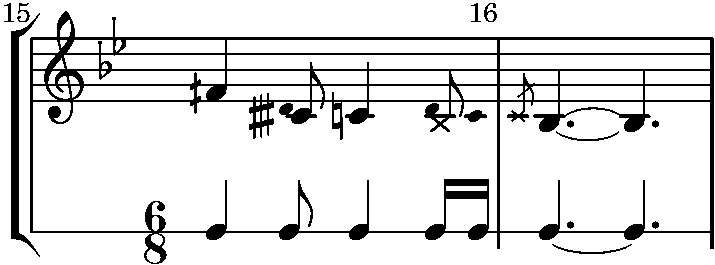
\includegraphics[width=0.65\linewidth]{deviation_example_2_mixed}
	\caption[Average tonal and rhythmic deviations]
		{Average deviations in the participants' performances in the universal lullaby.
		Smaller, stemless notes mark the correct notes where deviation occurred.
		Crossed-head notes mark those that deviate from the correct rhythmic pattern.}
	\label{snippet:deviation_example}
	\addcontentsline{lof}{section}{Snippet \thesnippet: Average tonal and rhythmic deviations}
\end{snippet}

\section{Segmental convergence to natural and synthetic stimuli}
\label{sec:convergence_to_natural_and_synthetic_stimuli}

After finding accommodation effects in \ac{hhi} (\cref{chap:conv_analysis}) and other vocal productions (\cref{sec:alignment_in_novel_and_familiar_sung_music}), the next step on the way to accommodation in \ac{hci} is to test whether similar effects can be found when humans interact with synthetic voices.
The motivation for such an experiment is boosted by the \ac{casa} paradigm \citep[][and cf.\ \cref{subsec:verbal_interaction}]{Nass1994computers, Nass2000machines}.
That is, if computer-based interlocutors can be perceived as social functions in communicative interaction, the question arises, therefore, whether socially-oriented effect such as accommodation would occur in \ac{hci} as well.
This assumption is made, whether explicitly or implicitly, in accommodative systems like those surveyed in \cref{sec:adaptive_spoken_dialogue_systems}.
A simplified version of this experiment using the same stimuli is replicated in \cref{sec:showcase} as a demonstration of an accommodative \ac{sds}.

\subsection{Experimental design}
\label{subsec:design_HCIConv}

\subsubsection{Target features}
\label{subsubsec:target_features_HCIConv}

Three features were examined in the study, as listed below.
Their variations have been defined as a two-way categorical distinction, even if one of them can be modified on a gradual scale.
Although these features may pass as light dialectical markers \citep{Mitterer2013regional}, they do not carry any difference in meaning, and are generally ascribed to personal preference and speaking style.

\begin{enumerate}
	\item \textbf{\textipa{[\c{c}]} vs.\ \textipa{[k]} at a word-final $\langle$-\textit{ig}$\rangle$} syllable
	
	These variations of the phoneme \textipa{[\c{c}]} are both common native speakers of German.
	Using one variation or the other does not change the meaning of the word, or any other property of it.
	Although it can be generally said that \textipa{[\c{c}]} is more used in the south and \textipa{[k]} in the north of Germany, they do not mark a specific dialect or socio-economic status.
	This \enquote{neutrality} makes this feature a good candidate, since changes in pronunciation should not occur due to the liking of one dialect or the other, or as an attempt to match a certain social status.
	It is noteworthy that the \textipa{[\c{c}]} variation is considered to be more standard, but still, both of the variations are accepted and people typically do not even notice which variation they and their interlocutors are using.
	In this experiment, we treat this feature as bi-categorical in nature.
	The very few instances of other fricatives, such as \textipa{[S]} and \textipa{[J]}, were counted as \textipa{[\c{c}]} as well, making the distinction practically between fricative and plosive realization.
	Here are two examples of sentences with this feature that were used as material for the experiment's stimuli (for the full list of stimulus materials, see \autoref{app:shadow_experiment_stimul}):
	
	\begin{enumerate}[label=\arabic{enumi}\alph*), ref=\arabic{enumi}\alph*.)]
		\item 
		\begin{tabulary}{\linewidth}{LLLLL}
			Der				& köni\textbf{\underline{g}} & hält				& 	eine	& Rede.\\
			\textit{The}	& \textit{king} 			 & \textit{held}	& \emph{a}  & \emph{speech}.\\
		\end{tabulary}
		\item
		\begin{tabulary}{\linewidth}{LLLLL}
			Ich 		& bin		  & süchti\textbf{\underline{g}} & nach 		& Schokolade.\\
			\textit{I}  & \textit{am} & \textit{addicted} 			 & \textit{to}  & \textit{chocolate}.\\
		\end{tabulary}
	\end{enumerate}
	
	\item \textbf{\textipa{[e:]} vs.\ \textipa{[E:]} realization of the mid-word grapheme \enquote{ä}}
	
	These two phonemes represent the two extremes of this feature's realization.
	However, vowel quality, as opposed to the \textipa{[\c{c}]} vs.\ \textipa{[k]} feature, it is not categorical (fricative vs.\ plosive), but rather gradual.
	That means that the actual realization can be anywhere between these two extremes.
	Despite the gradual nature of vowel quality, native speakers still perceive this feature as categorical (either \textipa{[e]} or \textipa{[E]}, cf.\ \citet{Kuhl2004early, Kuhl1991human}).
	In this experiment, we treat this feature as categorical in the first phase (see \cref{subsubsec:procedure_hci}), but measure it as gradual for analysis purposes (see \cref{subsec:results_hci}).
	This allows the detection of non-categorical changes over time, which are important for characterizing the convergence process.
	The \textipa{[E]} variation is in general more typical for the southern federal states of Germany, while \textipa{[e]} is more common in the north.
	As in the case of the \textipa{[\c{c}]} vs.\ \textipa{[k]} feature, the use of one realization or the other (or any in-between them) does not make any difference in meaning.
	Here are two examples of sentences with this feature that were used as material for the experiment's stimuli (for the full list of stimulus materials, see \autoref{app:shadow_experiment_stimul}):
	
	\begin{enumerate}[label=\arabic{enumi}\alph*), ref=\arabic{enumi}\alph*.)]
		\item 
		\begin{tabulary}{\linewidth}{LLLLL}
			War 		 & das 			& Ger\textbf{\underline{ä}}t & sehr			 & teuer?\\
			\textit{was} & \textit{the} & \textit{device}			 & \textit{very} & \textit{expensive}?\\
		\end{tabulary}
		\item
		\begin{tabulary}{\linewidth}{LLLLLL}
			Ich		   & mag 			& die 			& Qualit\textbf{\underline{ä}}t & deiner		   & Tasche.\\
			\textit{I} & \textit{like}  & \textit{the}  & \textit{quality} 				& \textit{of your} & \textit{bag}.\\
		\end{tabulary}
	\end{enumerate}
	
	\item \textbf{\textipa{[@n]} vs.\ \textipa{[\s{n}]} at a word-final $\langle$-\textit{en}$\rangle$ syllable}
	
	Unlike the two previous features, this feature does not, typically, show variation in -- all the more so in spontaneous speech, which is more relevant in the context of \acp{sds}.
	While the \textipa{[@n]} variation may occur when one wants to emphasize the word/syllable or when speaking more clearly, e.g., with children or when in a noisy environment, the \textipa{[\s{n}]} variation is by a large margin the more dominant one.
	It is rare to hear consistent production of a \textipa{[@n]} in an ending-syllable $\langle$-en$\rangle$.
	This is true across-dialects and regions, and it is ascribed to the phonological rule \textit{schwa elision} that occurs in the German language, as follows \citep[adapted from][pp.~142--143]{Benware1986phonetics}:
	%
	\begin{equation}
		\text{\textipa{@n}}\longrightarrow \varnothing \text{\textipa{\s{n}}} \diagup
		%	\left[\text{$-$son}\right] \ \_\_ \ \{\text{\#}, \left[\text{+const}\right]\} .
		\text{+consonantal} \ \_\_ \ \ \text{\#} .
		\label{eq:elision_rule}
	\end{equation}
	\eqname{Phonological process: Schwa elision in German}
	%	
	Here are two examples of sentences with this feature that were used as material for the experiment's stimuli (for the full list of stimulus materials, see \cref{app:shadow_experiment_stimul}):
	
	\begin{enumerate}[label=\arabic{enumi}\alph*), ref=\arabic{enumi}\alph*.)]
		\item 
		\begin{tabulary}{\linewidth}{LLLLL}
			Wir 		& besuch\textbf{\underline{en}} & euch 		   & bald 		   & wieder.\\
			\textit{We} & \textit{will visit} 			& \textit{you} & \textit{soon} & \textit{again}.\\
		\end{tabulary}
		\item
		\begin{tabulary}{\linewidth}{LLLLLL}
			Sind 		 & die 			& Küch\textbf{\underline{en}} & immer		    & so 		  & groß?\\
			\textit{Are} & \textit{the} & \textit{kitchens} 		  & \textit{always} & \textit{so} & \textit{big}?\\
		\end{tabulary}
	\end{enumerate}
\end{enumerate}

It is important to note, that although speakers may have their preferred variants in the contexts given in this study, \textipa{[E:]}, \textipa{[e:]}, \textipa{[Ik]}, \textipa{[\s n]}, and \textipa{[@n]} are all part of the phonetic inventory of native speakers of German and are used by all speakers in other contexts. 

\subsubsection{Procedure}
\label{subsubsec:procedure_hci}

The experiment consisted of three production phases (see \cref{fig:HCIConvFlow}): \emph{baseline} production, \emph{shadowing} task, and \emph{post} production.
In the baseline phase, the participants were asked to read out the stimuli from a monitor.
Each stimulus was presented separately with nothing else on the screen.
The participant's most frequent variant of each target feature (\cref{subsubsec:target_features_HCIConv}) was recorded.
No instructions whatsoever were given regarding the pronunciation of the sentences.
Then, in the shadowing task, the participants produced the stimuli sequentially, each after listening to another voice (either natural or synthetic, both male and female, see \cref{subsubsec:stimuli_participant_hci}) that used the opposite category of the relevant target feature.
For example, if a participant mostly produced \textipa{[\c{c}]}, the stimuli's realization of the \textipa{[\c{c}]} vs.\ \textipa{[k]} contrast was \textipa{[k]}.
Based on the production in this phase, the participant's tendency, pace, and degree of convergence were analyzed.
These analyses were are the basis for the model presented in \cref{chap:computational_model}.
Finally, in the post phase, the participant once again read out the stimuli from a screen.
The purpose of this phase was to examine whether a convergence effect was maintained when the external input is absent.
Between the baseline and shadowing productions, the participants had a break of about seven minutes.
Its purpose was to let the mental representation of the production fade, so that the base production will not influence as much on the productions in the following parts.
To boost this process, the participants played a game with strong visual aspects and with non-verbal sounds only.
Conversing with the participant was avoided as much possible as possible in order to prevent other verbal input from influencing their mental representations.
The participants' performance in the game was not recorded and did not influence the next parts in any way.
%
\begin{figure}[t]
	\centering
	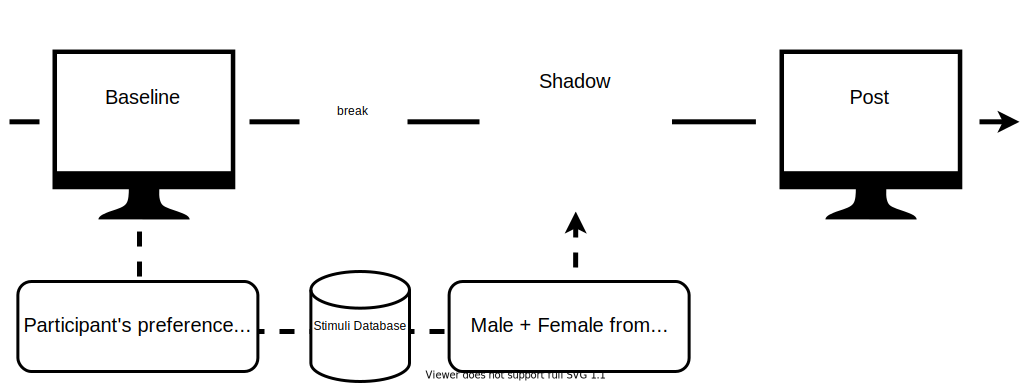
\includegraphics[width=\linewidth]{HCI_flow}
	\caption[\acs{hci} convergence experiment workflow]
		{Flow of the experiment (from left to right).
		Stimuli are read from a monitor in baseline and post phases, while heard over headphones in the shadowing task.
		The participant's preferred variation recorded in the baseline productions are used to select those with the opposite realizations from the stimuli database for the shadowing task.
		Each participant listened to both male and female voices of one of the stimulus types natural, diphone, or \acs{hmm}.}
	\label{fig:HCIConvFlow}
\end{figure}
%
A program developed specifically for the purpose of this experiment was used for its execution.
It included functionalities tailored for this experiment and a \ac{gui} the experimenter could use during the and between the phases to quickly record participants' performance and prepare the next phase.
These include setting up the participants' audio streams (e.g., playback and recording volumes), extracting the appropriate stimuli from the database, semi-randomizing the stimuli into balanced groups, logging the timing and participants' productions, and more.
The experiment was carried out in a sound-proof booth located inside a recording studio.
Seeing that the experiment dealt with the way people change their way of speaking based on the speech of others, conversation with participants was kept to a minimum before the experiment and was avoided till the end of the experiment.
%It goes without saying, however, that it was not realistic to try and control for any kind of conversation the participants might have had during the day prior to the experiment.

\subsubsection{Stimuli and participants}
\label{subsubsec:stimuli_participant_hci}

As mentioned above, shadowing experiments are common practice in accommodation studies.
However, this is typically done with single words as targets or with a repeating carrier sentence.
Unlike those experiments, in the experiment presented here, participants shadowed full sentences instead of single, typically mono- or bisyllabic (non-)words.
Each of the three target features was represented in three declarative and two interrogative grammatical German sentences, five to seven words long.
Additionally, 25 filler sentences, in which none of the target features occur, were introduced as a control mechanism and to not make the target features too obvious.
At the beginning of the baseline phase, five additional filler sentences were shown to let the participant get used to the task and the setting.
Three sets of stimuli were created (one natural and two synthetic), leading to a total of 270 stimuli ((3 features $\times$ 5 sentences + 25 fillers + 5 warm-ups) $\times$ 3 sets $\times$ 2 genders).
One set of stimuli was created with the (natural) speech of one female and one male native German speakers from the same age group of most participants -- 25 and 23 years old, respectively.
As for the synthetic stimuli, there are multiple synthesis methods to choose from:
Formant synthesis \citep[e.g.,][]{Burkhardt2000verification}, unit selection \citep{Hunt1996unit,Black2003unit}), diphone synthesis \citep[e.g.,][]{Dutoit1996mbrola}, and probabilistic (e.g., using \acp{hmm} as described in \citet{Zen2005overview} and in \citet{Zen2009statistical}), to name some.
Diphone synthesis using \acl{mbrola} \citep[\acs{mbrola};][]{Dutoit1996mbrola} and probabilistic \ac{hmm} synthesis were selected for creating this experiment's stimuli, due to their combination of control over pronunciation and overall quality.
One stimulus set including both male and female voices was created with each of these methods.
These three sets were stored in a database that was used in the shadowing phase of the experiment (see \cref{fig:HCIConvFlow}).
A more advanced technique, like the neural \ac{s2s} used in \cref{subsec:speech_manipulation}, was not selected due to its lack of direct control over specific segments and to avoid voices resembling natural too much natural voices.
To better focus on segmental differences, suprasegmental properties in the synthetic stimuli were fixed to match those of the natural utterances.
This was done separately for male and female voices with the respective human speakers.
The \ac{f0} contour (and by extension also stresses) and segment lengths (and by extension also speech rate) of each sentence of the natural stimuli were imposed on the synthetic stimuli in both synthesis methods \citep[and see][]{Raveh2017ESSV}.
%
\begin{figure}[t]
	\centering
	\subfigure[\ac{f0} contour of the natural production]
		{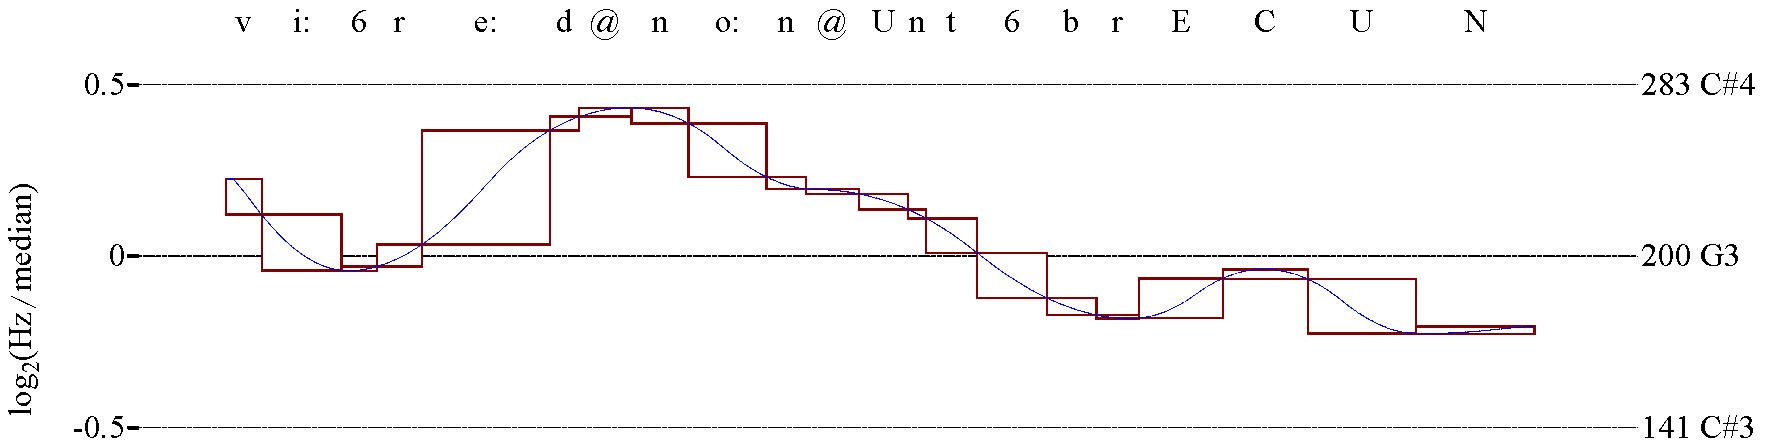
\includegraphics[width=\textwidth]{momel-natural}
	\label{fig:momel-natural}}
	\subfigure[synthetic stimulus with imposed \ac{f0} from the natural production]
		{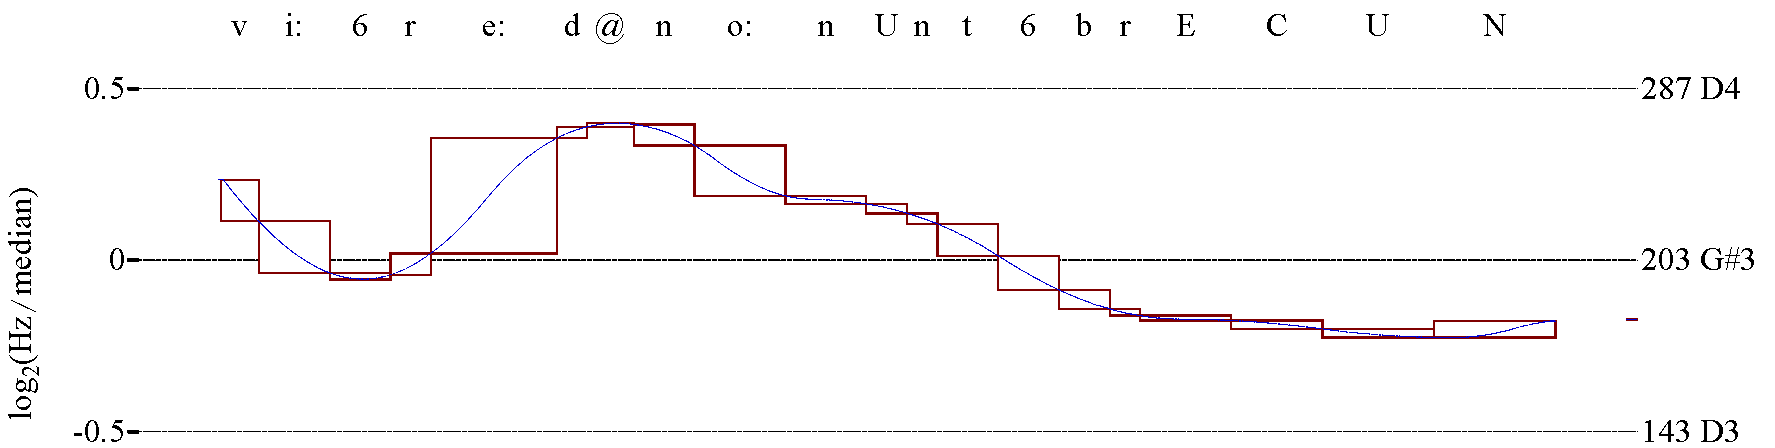
\includegraphics[width=\textwidth]{momel-synthetic}
	\label{fig:momel-synthetic}}
	\caption[MOMEL comparison of natural \acs{f0} contour imposition on a synthetic stimulus]
		{MOMEL-INTSINT contours of the natural stimulus (top) and its corresponding MBROLA synthetic stimulus (bottom) for the sentence \emph{\enquote{Wir reden ohne Unterbrechung}} with corresponding SAMPA transcriptions.
		The numeric and alphanumeric values to the right are the absolute pitch frequencies and their corresponding musical tone.
		The scale to the left displays one octave around the median pitch of the signal.}
	\label{fig:momel-comparison}
\end{figure}
%
With \ac{mbrola} this process is straightforward, as the duration and pitch values can be directly passed as input.
For the \ac{hmm} synthesis, the process was more complex.
To predict voiceness, the mel-generalized cepstra and band aperiodicity coefficients were first extracted from the spectrum of the output signal of the regular HTS process.
Subsequently, A neural network with a hidden layer of 128 neurons was used to predict the voicing property from the cepstra coefficients.
Then, a voicing mask was applied to the imposed \ac{f0} contour to obtain the final \ac{f0} coefficients.
Finally, All the coefficients were used to generate the output signal in a standard synthesis chain with a mel log spectrum approximation filter and the STRAIGHT vocoder \citep{Kawahara2006straight}.
%The descriptive features and question sets used to build the decision tree followed the standard English set proposed in [17] with adapted part-of-speech tags and phonemes for German. 
%These values were extracted from the annotations of the natural stimuli (see \citet{Gessinger2016PundP}):
The segment lengths were directly taken from the annotations, and the \ac{f0} contours were acquired by first interpolating the contour of the natural stimuli and then record the \ac{f0} value at the beginning and the middle of each segment.
It goes without saying, however, that due to the limitations of the synthesis techniques, the generated contours were not always \emph{completely} identical to those of the corresponding natural stimuli, as shown in \cref{fig:momel-comparison}.
Nevertheless, no substantial differences in overall sentence intonation or stress were introduced.

\begin{table}[t]
	\centering
	\caption[Summary of participant in the \acs{hci} experiment]
		{Summary of participant characteristics listening to each stimulus set.}
	\label{tab:participants_hci}
	\begin{tabulary}{\linewidth}{LSLSS}
		\toprule
		\textbf{condition} & \multicolumn{2}{c}{\textbf{no.\ of participants}} & \textbf{age range} & \textbf{mean age}\\
		\midrule
		\multirow{2}{*}{Natural} & 17 & female & \numrange{19}{33} & 26 \\
	 			& 4  & male   & \numrange{23}{34} & 30 \\
		\rule{0pt}{0.4cm}%
		\multirow{2}{*}{Diphone} & 14 & female & \numrange{19}{50} & 26 \\
	 			& 4  & male   & \numrange{23}{34} & 27 \\
		\rule{0pt}{0.4cm}%
		\multirow{2}{*}{HMM} 	& 13 & female & \numrange{18}{51} & 28 \\
	 			& 4  & male   & \numrange{22}{37} & 25 \\
		\bottomrule
	\end{tabulary}
\end{table}
%
56 native German speakers from ten different states in Germany took part in the experiment.
Three non-overlapping subgroups listened to the three stimulus sets.
In a post-experiment questionnaire, \SI{80}{\percent} of the participants indicated that change the way they speak depending on their interlocutor, \SI{50}{\percent} believed they would converge to an interlocutor of the same dialectal background, and \SI{15}{\percent} claimed they would converge to an interlocutor from a different dialectal background.
Each participant was presented with only one of the three stimulus types.
\Cref{tab:participants_hci} shows a detailed overview of the participants.
Importantly, the age of the human speakers that recorded the natural stimuli match the mean age of all participants.
As explained in \cref{subsubsec:procedure_hci}, the participants' preference for each of the target features was obtained in the baseline phase.
These preferences are summarized in \cref{tab:preference_hci}.
At the end of the experiment, the participants were asked which realization of each feature they believe to produce themselves and what they think of the other version of it.
About \SI{75}{\percent} reported a positive attitude towards the version they \emph{do not} believe to produce themselves.
Only a minority of participants showed a negative attitude towards the other variation.
Based on the results (see \cref{subsec:results_hci}, it seems therefore plausible that a positive attitude towards the features entails a higher probability of converging to them.
%
\begin{table}[t]
	\centering
	\caption[Summary of participants' preference in the \acs{hci} experiment]
		{Summary of participants' preferred realization of each target feature based on productions in the baseline phase.}
	\label{tab:preference_hci}
	\begin{tabulary}{\linewidth}{LSSSSSS[table-format=1.0]}
		\toprule
		\textbf{condition} &
		\multicolumn{2}{l}{\textbf{\textipa{[E:]} vs.\ \textipa{[e:]}}} &
		\multicolumn{2}{l}{\textbf{\textipa{[I\c{c}]} vs.\ \textipa{[Ik]}}} &
		\multicolumn{2}{l}{\textbf{\textipa{[\s{n}]} vs.\ \textipa{[@n]}}}\\
		\midrule
		Natural & 11 & 10 & 12 &  9 & 21 & 0 \\
		Diphone & 14 &  4 &  9 &  9 & 17 & 1 \\
		HMM     & 10 &  7 &  6 & 11 & 16 & 1 \\
		\bottomrule
	\end{tabulary}
\end{table}

\subsection{Analyses and results}
\label{subsec:results_hci}

The occurrences of each feature were analyzed separately.
The feature \textipa{[E:]} vs.\ \textipa{[e:]} was evaluated as a continuum in the F1-F2 formant space.
%Automatic annotations (WebMAUS, \cite{Kisler/etal:2017}) of all target vowel segments were manually corrected by a trained phonetician.
The first and second formants of each target segment were measured at the temporal midpoint in all productions as well as in the stimuli using Praat \citep{Boersma2018praat}. 
These values were used for calculating the Euclidean distance between the participants' and stimuli vowel realizations in each sentence using the formula
%
\begin{equation}
	E_{dist}=\sqrt{(F1_{participant}-F1_{model})^2+(F2_{participant}-F2_{model})^2}.
\end{equation}
\eqname{Euclidean distance in F1-F2 space}
\noindent
%
Smaller distance in the shadowing or post phases compared to the baseline phase points to a convergence effect.
\Cref{fig:ee_E_space} illustrates the convergence effects as realized by one of the participants.
The distances were measured using the mean values of all stimuli in the set to which the participant listened.
These distances were used to fit linear mixed-effects models with phase as a fixed effect, subject and target word as random effects (intercepts and slopes), and distance as the dependent variable.
Models were fit for both preference groups compared by an ANOVA.
The differences between baseline and shadow phases were found to be significant in the natural and \ac{hmm} groups, and between the baseline and post phases only in the natural group.
\Cref{tab:lmm_ee_E} summarizes the results for this feature.
\Cref{fig:ee_E_space} provides additional insights regarding the perception of the vowel quality contrasts in the synthetic stimuli due to their realization in these sets.
The influence of the production overlaps is discussed in \cref{sec:conclusion_shadowing}.
%
\begin{table}[t]
	\centering 
	\caption[Convergence results for \textipa{[E:]} vs.\ \textipa{[e:]} with three stimuli sets]
		{Summary of convergence effects between the three phases.} 
	\label{tab:lmm_ee_E} 
	\sisetup{table-format=3.2, parse-numbers=false}

	\begin{tabularx}{\linewidth}{XSSS}
		\toprule
		\textbf{Natural} & \multicolumn{1}{c}{\textbf{base-shadow}} & \multicolumn{1}{c}{\textbf{base-post}} & \multicolumn{1}{c}{\textbf{shadow-post}}\\
		\midrule
		intercept           & 69.94\textsuperscript{***}		& 32.88    	& $-$33.67\textsuperscript{**} \\
                         	& (14.89)  		& (17.53)  	& (11.44)     	\\
		\textsc{preference}	& 33.79\textsuperscript{*}		&          	&             	\\
                         	& (14.89)     	&          	&             	\\
 		\midrule
		observations 		& 210 			& 210 		& 209 			\\ 
		\bottomrule
	\end{tabularx}	

	\begin{tabularx}{\linewidth}{XSSS}
		\toprule
		\textbf{Diphone} & \multicolumn{1}{c}{\phantom{\textbf{base-shadow}}} &
        \multicolumn{1}{c}{\phantom{\textbf{base-post}}} &
        \multicolumn{1}{c}{\phantom{\textbf{shadow-post}}} \\
		\midrule
		intercept           & $-$1.68  	& $-$1.49  	& 0.44   \\
                        	& (8.72)   	& (9.93)   	& (7.24) \\
% 		\midrule
%		observations 		& 177 		& 179 		& 178    \\ 
		\bottomrule
	\end{tabularx}
	
	\begin{tabularx}{\linewidth}{XSSS}
		\toprule
		\textbf{\ac{hmm}} & \multicolumn{1}{c}{\phantom{\textbf{base-shadow}}} &
        \multicolumn{1}{c}{\phantom{\textbf{base-post}}} &
        \multicolumn{1}{c}{\phantom{\textbf{shadow-post}}} \\
		\midrule
		intercept      	& 32.64\textsuperscript{*} 	& $-$2.12  	& $-$31.23 \\
                       	& (13.61)  	&(12.38)  	& (15.86)  \\
% 		\midrule
%		observations 	& 134 		& 135 		& 133      \\ 
		\bottomrule
		\multicolumn{4}{l}{\small{$^{***}p<0.001$, $^{**}p<0.01$, $^*p<0.05$}}
	\end{tabularx} 
	\todo[inline]{to fix: numbers in table are not perfectly aligned because of parentheses}
\end{table} 
%
\begin{figure}[t]
	\centering
	\begin{minipage}{.47\linewidth}
		\centering
		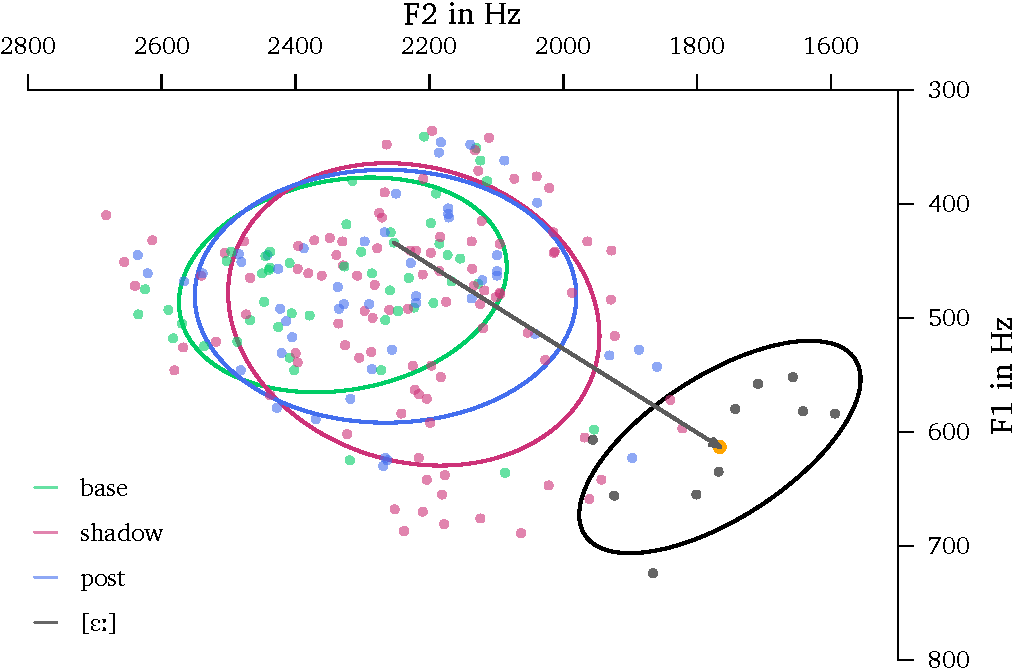
\includegraphics[width=\linewidth]{ee_E_space}
		\caption[Example of vowel quality convergence towards a model speaker]
			{An example of a participant's vowel quality convergence towards the stimuli.
			The participant's preference is \textipa{[e:]} while the variation \textipa{[E:]} is used in the stimuli (and cf.\ \cref{fig:ee_E_circles}).
			The colors of the circles represent the {\color{base-green}\textbf{base}}, {\color{shadow-red}\textbf{shadow}}, and {\color{post-blue}\textbf{post}} phases, and the model's formant values with $\pm1$ standard deviation from the bivariate mean.
			The arrow shows the distance between one of the participant's production and the {\color{model-orange}\textbf{model mean}}.}
		\label{fig:ee_E_space}
	\end{minipage}
	\hfill
	\begin{minipage}{.47\linewidth}
		\centering
		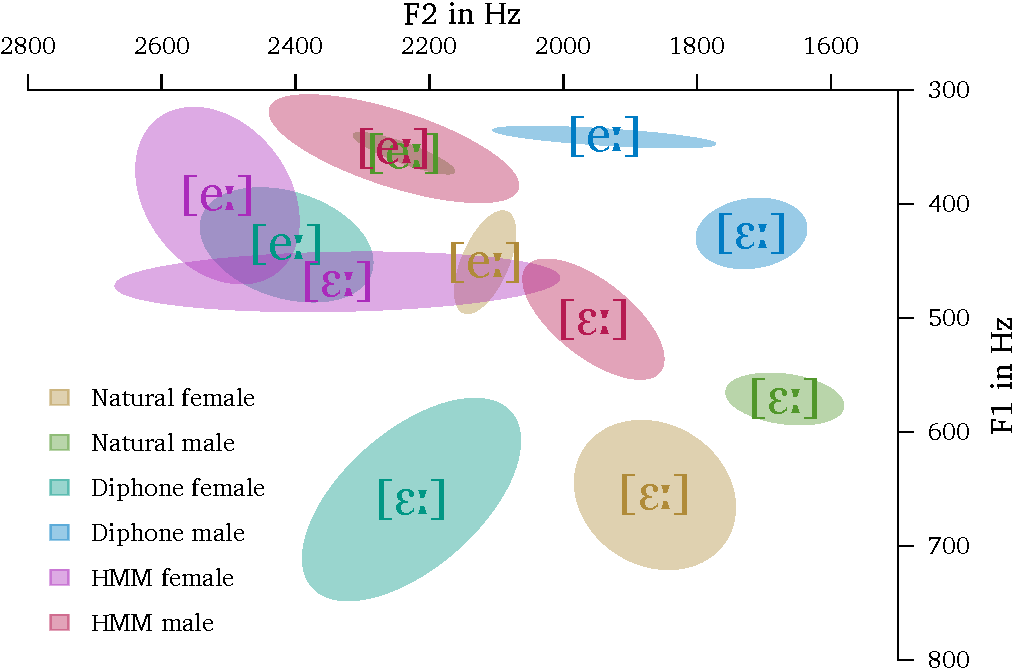
\includegraphics[width=\linewidth]{ee_E_circles}
		\caption[F1 and F2 value areas of all stimulus groups]
			{Values areas of the first two formants of the three stimulus sets' \textipa{[e:]} and \textipa{[E:]} instances.
			 Each color represents both male and female ranges of on stimulus type (natural, diphone, or \ac{hmm}).
			 The smaller a circle is, the more well-defined the mean target of this stimulus group is.
			 Moreover, the further apart circles of the same color are, the more distinct the difference is within this set.}
		\label{fig:ee_E_circles}
	\end{minipage}	
\end{figure}

The \textipa{[I\c{c}]} vs.\ \textipa{[Ik]} was evaluated based on the percentage of same-category realizations of the participants with respect to the stimulus set they listened to.
If the percentage increased, e.g., between baseline and shadow productions, the participant converged to the stimuli.
\Cref{fig:ic_ik_results} summarizes the per-phase differences for each set.
With all three data sets combined, the number of same-variant productions increased by about \SI{30}{\percent} from the baseline phase to the shadowing phase, and decreases again in the post phase, but to a lesser degree.
That means that all in all, participants not only converged to the stimuli in the shadowing phase, but the effect lasted to some extent in the post phase as well.
The statistical significance between the phases within each stimulus type was tested using a Gaussian linear mixed-effects model.
For both the natural and diphone sets, the increases between the baseline and the shadowing phases were significant, \SI{10}{\percent} to \SI{39}{\percent} and \SI{16}{\percent} to \SI{48}{\percent}, respectively.
Moreover, in these sets, the decreases in the post phase did not go all the way to the baseline level: \SI{39}{\percent} to \SI{23}{\percent} for the natural set and \SI{48}{\percent} to \SI{36}{\percent} for the diphone set.
For the \ac{hmm} set, the increase between baseline and shadowing was \SI{8}{\percent} to \SI{40}{\percent} and did not reach the significance threshold.
However, the decrease in the post phase reached the baseline level again and was significant, from \SI{40}{\percent} to \SI{12}{\percent}.
%
\begin{figure}[t]
	\centering
	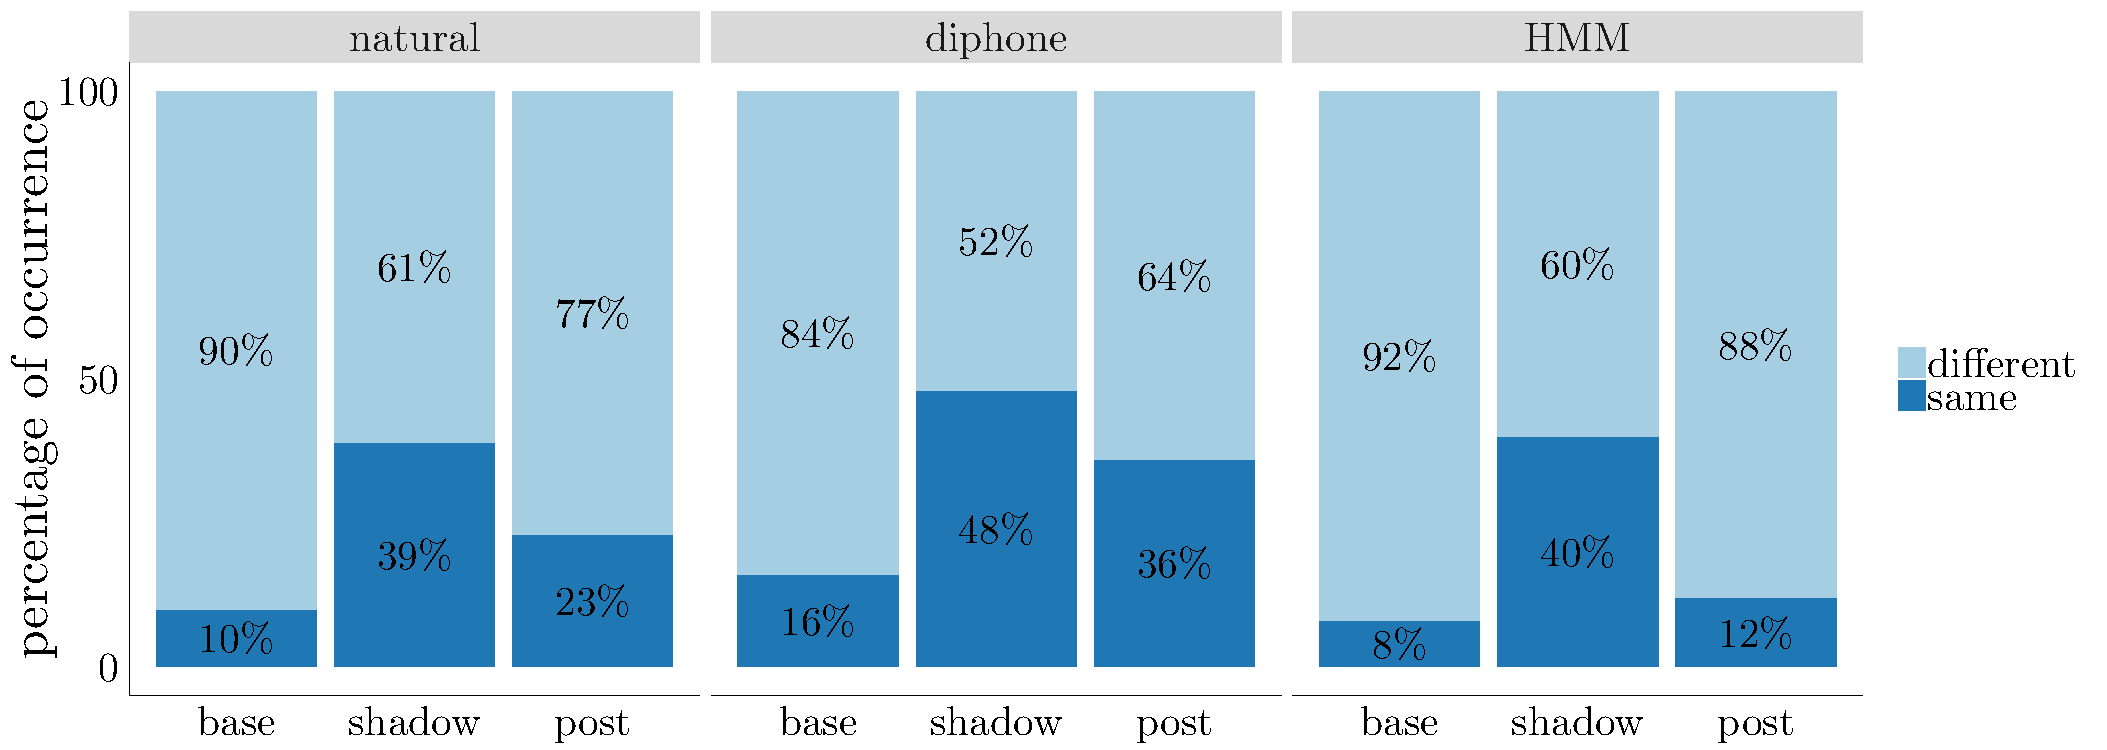
\includegraphics[width=\textwidth]{ic_ik_results}
	\caption[Convergence results for \textipa{[I\c{c}]} vs.\ \textipa{[Ik]} with three stimuli sets]
		{Percentage of same-variant and different-variant realization of participants with respect to the stimulus type they listened to in the shadowing phase.
		An increase between the base and the shadow phases indicates convergence towards the stimuli.
		Similarly, the decrease between the shadow and the post phases back towards the baseline level shows the degree to which the convergence effect remained when the stimuli were not present anymore.}
	\label{fig:ic_ik_results}
\end{figure}
%

The \textipa{[\s{n}]} vs.\ \textipa{[@n]} was measured based on the lengths of the potential schwa segments in the sentences.
To decide whether schwa was present or absent in the participants' target word productions, the lengths of relevant segments between the preceding consonant -- \textipa{[d], [t], [\c{c}], [x], or [f]} -- and the final nasal were measured.
A duration of \SI{30}{\milli\second} was established as the threshold of a perceived schwa segment.
This decision is also supported by the fact that all schwas occurrences in the stimuli sets were at least \SI{30}{\milli\second} long.
The segment length range of the natural stimuli, along with the lengths' variance of the participants' productions, is shown in \cref{fig:schwa_conv_bars}.
Note that only two participants showed a preference toward the \textipa{[@n]} variant in their baseline productions (cf.\ \cref{tab:preference_hci}).
This indicates that schwa does not commonly appear in the examined context, which might make it harder to trigger convergence among the participant.
Seeing that a statistical analysis for a group of two participants is likely to be misleading, these participants were excluded from the analysis of this feature.
\Cref{tab:schwa_results} summarizes the percentage of schwa occurrences in the three phases.
There was an increase of schwa occurrences between the baseline and shadowing phases for all stimulus types, with the difference being significant for the natural and \ac{hmm} sets with changes of \SI{9}{\percent} and \SI{5}{\percent}, respectively.
In the post production, the number of schwa occurrences decreased to approximately the baseline level for all conditions.
Interestingly, while for the natural stimuli this decrease was still above the baseline percentage, for both the synthetic sets the percentage in the post phase was even lower than in the baseline phase.
%
\begin{figure}[t]
	\begin{minipage}{.48\linewidth}
			\centering
			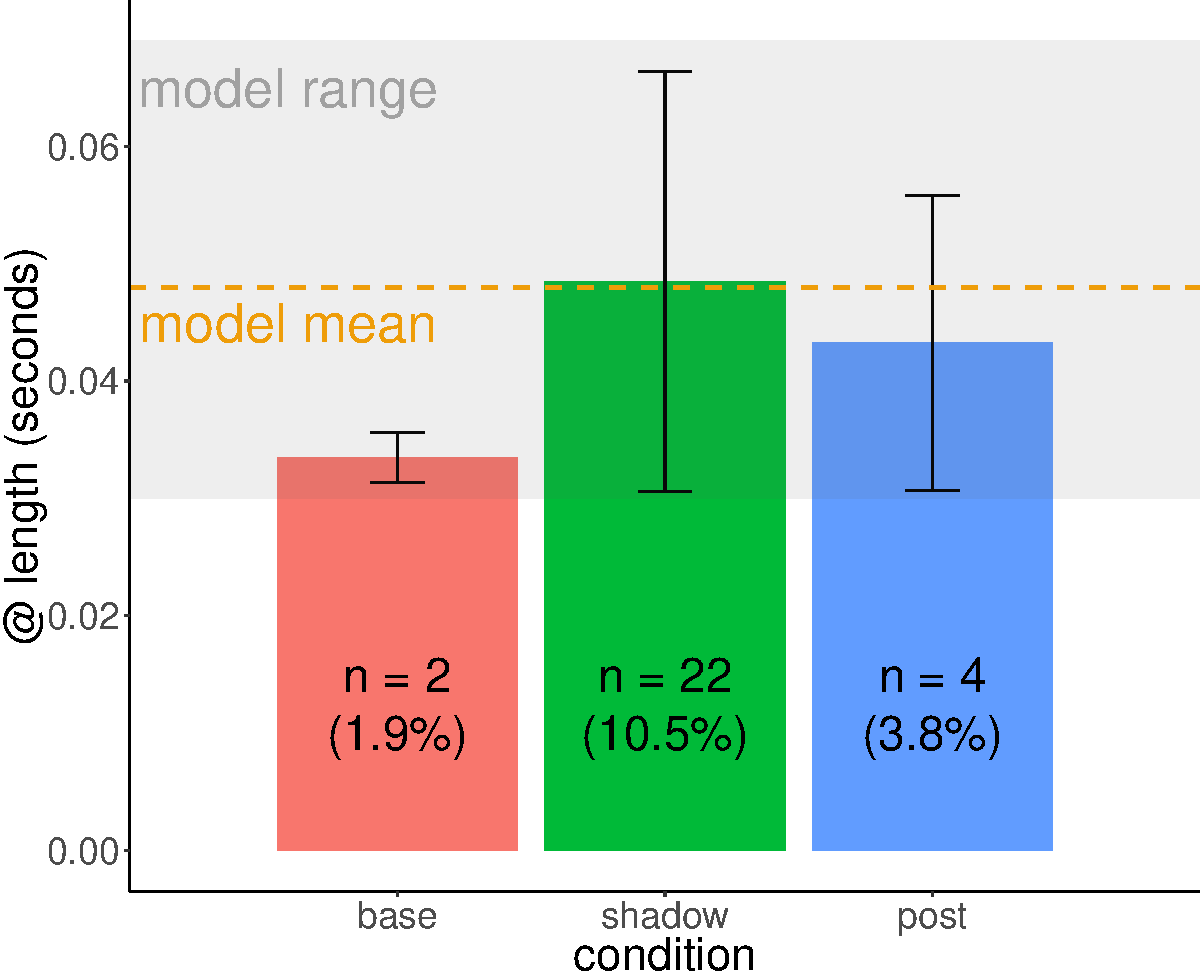
\includegraphics[width=\textwidth]{schwa-plot}
			\caption[Illustration]
				{Schwa segment lengths in the three phases.
				 The height of each bar represents the average length in this phase, and the corresponding whiskers indicate the overall value range.
				 The gray area shows the value range of the stimuli, with the mean length at the orange dashed line.}
			\label{fig:schwa_conv_bars}
	\end{minipage}
	\hfill
	\begin{minipage}{.49\linewidth}
			\centering
			\captionsetup{type=table}
			\caption[Convergence results for \textipa{[\s{n}]} vs.\ \textipa{[@n]} with three stimuli sets]
				{Percentage of schwa occurrences in each phase and stimulus set.
				 $N$ stands for the number of sentences with the target feature \textipa{[\s{n}]} vs.\ \textipa{[@n]}, which is derived from the number of participant with \textipa{[\s{n}]} preference (the shadowing phase always has double the number of sentences, because both male and female voices were used).}
			\label{tab:schwa_results}
			\begin{tabularx}{\linewidth}{lccc}
				\toprule
				& \textbf{base} & \textbf{shadow} & \textbf{post} \\
				\midrule
				\multirow{2}{1.4cm}{Natural}	& \SI{1.9}{\percent} & \SI{10.9}{\percent} & \SI{3.8}{\percent}  \\\vspace{0.3cm}
											& $ N = 105 $ 		 & $ N = 210 $		   & $ N = 105 $		 \\
				\multirow{2}{1.4cm}{Diphone} 	& \SI{2.4}{\percent} & \SI{4.1}{\percent}  & \SI{1.2}{\percent}  \\\vspace{0.3cm}
											& $ N = 85 $ 		 & $ N = 170 $ 		   & $ N = 85 $			 \\
				\multirow{2}{1.4cm}{\acs{hmm}} 	& \SI{2.5}{\percent} & \SI{7.5}{\percent}  & \SI{1.25}{\percent} \\
											& $ N = 80 $ 		 & $ N = 160 $ 		   & $ N = 80 $			 \\
				\bottomrule
			\end{tabularx}
	\end{minipage}
\end{figure}

\section{Conclusion}
\label{sec:conclusion_shadowing}

The results found in the music experiment show that alignment occurs in singing, more so with respect to temporal features than to tonal ones.
This stands in contrast to findings in interactive speech \citep[e.g.,][]{Raveh2019InterspeechAlexa}).
Even so, the results emphasize the similarity between the two oral capabilities, viz.\ speech and singing, which are both used in human communication.
They are therefore also prone to influence each other and can potentially be related and enhance one another.
For example, \citet[][p.\ 216]{Nardo2009musicality} explain that \emph{tonal} and \emph{rhythmic} abilities are measures of musicality and also related to phonetic talent.
This idea is also supported by \citet{Tsang2018musical}, who found a correlation between musical experience and sensitivity to convergence.
Similarly, pitch has been found to correlate with the level of agreement between interlocutors in dyadic conversation \citep{Okada2012interpreting}.
We therefore suggest that speech and music are two domains where certain common effects, and in particular convergence, occur with respect to shared prosodic features.
Establishing this connection between music and speech offers a wide range of further interdisciplinary experimentations that combine linguistic and musical analysis methods.
Specifically for convergence, the influence of listening to people with different social and vocal characteristics can be examined.
The manner in which distances in vocal behavior decrease, or increase, can depend on further aspects of the social environment and auditory context, as suggested by \citet{Noy1999psychoanalysis}.
To sum up, the first hypothesis -- convergence to perceived musical stimuli -- was satisfied, but not in the same way for pitch and tempo.
While tempo became globally closer to the recorded version in absolute terms, the tones were produced more precisely but within the same tonal range.
Additionally, the secondary expectation was only partially met, with fewer large deviations occurring in the shadowing performances, but otherwise the tones in the baseline production were slightly more accurate as a whole.
Finally, the third hypothesis was fulfilled, as the simpler, frequent rhythmic patterns were replicated more correctly.
Furthermore, with one exception, participants were not able to replicate the entire lullaby.
Interestingly, they remembered either part A or B, but did not mix bars from both.

As for the \ac{hci} experiment, different degrees of convergence were found for each of the three target features.
The feature \textipa{[E:]} vs.\ \textipa{[e:]} showed a convergence effect in all stimulus sets, but only in the natural set this effect was significant.
The areas covered by each vowel in \cref{fig:ee_E_circles} sheds light on possible reasons for the overall worse performance of the synthetic stimuli.
First, the vowels of the same category from the male and female diphone voices occupy a much larger area than those from the male and female natural voices, which results in a less distinct convergence target.
And second, all instances that are supposed to be \textipa{[E:]} in the female \ac{hmm} voice are located in the area of \textipa{[e:]}.
Hence, in the \ac{hmm} condition, all participants with preference \textipa{[e:]} actually heard their preferred version of the vowel in half of the trials during the shadowing phase.
These lead to the conclusion that the lack of a stronger effect could be due to the acoustic properties of the target vowels in the synthetic stimuli and not necessarily to the synthetic nature of the stimuli itself.
The feature \textipa{[I\c{c}]} vs.\ \textipa{[Ik]} was found to be a consistent trigger of phonetic convergence.
For all three stimulus types, the participants produced the opposite variant than their preference in roughly a third of the trials.
These cases of convergence do not only stem from participants that already showed both target forms in the baseline production, but also from participants that produced only one of the two forms in the baseline phase.
This a strong effect compared to the other two target features.
It might be explained by the fact that this feature is categorical by definition, as opposed to the other features which have two defined categories but are realized on a continuum (formant values and segment length).
The feature \textipa{[\s{n}]} vs.\ \textipa{[@n]} showed a rather small convergence effect.
This was expected, as schwa is not usually produced in the word-final sequence \textit{-en}.
Nevertheless, in all three conditions more instances of schwa were produced during the shadowing phase than in the baseline and post phase.
These productions are mostly attributable to one or two participants per condition who responded even to this unusual segmental feature.
This leads us to observe that apart from the identified group differences, the overall degree of convergence varied considerably among the participants, with some being \enquote{resistant} to external influence and others responding strongly to them.
In conclusion, it can be summarized that humans do indeed converge phonetically when interacting with synthesized speech. 
However, the degree of convergence depends on the nature of the target feature. 
The perceptibility of the target feature in the stimuli is proposed as a possible explanation for the fact that one of the examined features did not show the same extent of convergence for the synthetic stimuli as for the natural ones.

The two shadowing studies presented here show that vocal accommodation can also be found in a controlled experimental environment as part of a quasi-conversational scenario.
As a continuation of the effects found in \cref{chap:conv_analysis}, these results demonstrate that vocal accommodation occurs also in non-speech and human-computer settings.
These -- and especially the latter -- prove that accommodation effects are not exclusive to \acp{hhi} and thus lay the foundations for further investigation in \ac{hci}.
In chapter \cref{chap:speech_variations_in_hhci}, accommodation toward a computer-based interlocutor is examined in conversational, goal-oriented tasks.
The great individual differences found in these experiments inspired part of the parameters and approaches used in \crefrange{chap:computational_model}{chap:statistical_model}.
Their importance lies in the ability to give different \enquote{characters} (or \emph{profiles}, see \cref{subsec:accommodation_levels}) based on different human behavior, rather than letting a system behave the same in every interaction.
Furthermore, showing that convergence can occur in segmental features as well emphasizes the importance of control over such properties in synthetic speech for triggering vocal accommodation, which is attributed mostly to \ac{hhi}.
The segmental manipulations demonstrated in \cref{subsec:speech_manipulation} show how such differences can be achieved.